\documentclass[conference]{IEEEtran}
\IEEEoverridecommandlockouts

\usepackage{cite}
\usepackage{amsmath,amssymb,amsfonts}
\usepackage{algorithmic}
\usepackage{graphicx}
\usepackage{textcomp}
\usepackage{xcolor}
\usepackage{booktabs}
\usepackage{array}
\usepackage{float}
\usepackage{url}

\graphicspath{{../../ml/artifacts/report_figures/}{../../ml/artifacts/tsne/}{../../ml/charts/}{screenshots/ch3_current_2026_06_24/}}

\def\BibTeX{{\rm B\kern-.05em{\sc i\kern-.025em b}\kern-.08em
    T\kern-.1667em\lower.7ex\hbox{E}\kern-.125emX}}

\begin{document}

\title{Lightweight Vietnamese Speech Anti-Spoofing on Android:\
A Cross-Scale Attention Approach with Domain-Adaptive Feature Engineering}

\author{
\IEEEauthorblockN{Nguyen Kim Ngan}
\IEEEauthorblockA{\textit{Academy of Cryptography Techniques}\\
Hanoi, Vietnam}
\and
\IEEEauthorblockN{Duc-Tho Mai}
\IEEEauthorblockA{\textit{Academy of Cryptography Techniques}\\
Hanoi, Vietnam}
}

\maketitle

\begin{abstract}
Voice authentication is increasingly deployed in mobile and online services, but it is vulnerable to replay, text-to-speech, and voice conversion attacks. This risk is more acute for Vietnamese speech because publicly documented anti-spoofing systems are typically optimized for server-side inference and non-Vietnamese corpora rather than lightweight on-device deployment. This paper presents a practical Android-oriented pipeline that combines eight handcrafted acoustic features with a Cross-Scale Attention Lite classifier and a simple selective domain-mixing strategy. On an external Vietnamese holdout set of 1{,}700 samples, the proposed system reaches 85.29\% accuracy, 97.65\% spoof recall, and 86.91\% F1-score after mixing only 150 external samples per class into training. The final TensorFlow Lite model is 42.2 KB and the complete Android pipeline runs in 311 ms with 14.7 MB RAM, showing that effective Vietnamese speech anti-spoofing is feasible on commodity Android devices.
\end{abstract}

\begin{IEEEkeywords}
speech anti-spoofing, presentation attack detection, Android deployment, Vietnamese speech, handcrafted audio features, domain adaptation
\end{IEEEkeywords}

\section{Introduction}

Voice interfaces are now common in banking support, mobile assistance, and remote identity workflows, yet the same convenience widens the attack surface for synthetic and replayed speech. Recent progress in speech synthesis and voice conversion has made forged audio more natural, cheaper to generate, and harder to reject by human listening alone. As a result, a practical anti-spoofing system must detect attacks automatically, operate with low latency, and preserve privacy by avoiding mandatory cloud transmission.

These requirements are particularly demanding for Vietnamese speech. Vietnamese is tonal and acoustically diverse, but public anti-spoofing literature is still dominated by English-centric benchmarks and heavy spectrogram models. At the same time, Android deployment adds another constraint: the detector must run on CPU-only hardware, within limited memory, and without long feature-extraction pipelines. A design that succeeds on a GPU workstation may still be unusable in an everyday mobile application.

Prior work has shown strong anti-spoofing performance with end-to-end or graph-attention architectures such as RawNet2, RawBoost-based systems, and AASIST \cite{b1,b2,b3,b4}. However, those approaches are usually built around richer time-frequency inputs and larger runtime budgets. In our project setting, direct on-device execution required a smaller representation that remains discriminative under domain shift between internal training data and external Vietnamese samples.

The central intuition of this work is that spoofed and genuine Vietnamese utterances still differ in a set of low-cost statistical signatures. Synthetic samples tend to exhibit unnaturally stable amplitude envelopes, normalized peaks near full scale, and reduced pauses, while replayed or re-generated signals may show abnormal crest factors, clipping behavior, and altered active speech duration. These patterns can be summarized by a compact handcrafted vector, then classified by a lightweight attention model instead of a large spectrogram backbone.

The contributions of this paper are summarized as follows:
\begin{itemize}
    \item We design an eight-feature acoustic representation tailored for mobile inference, covering energy, instantaneous sign variation, dynamic range, clipping, and speech activity cues with very low computational overhead.
    \item We adapt a Cross-Scale Attention Lite classifier to low-dimensional feature vectors and show that it offers a better deployment trade-off than AASIST Lite and CBAM-ResNet Lite in our Android-oriented benchmark.
    \item We validate a simple domain adaptation strategy based on mixing only 150 external samples per class into training, which substantially improves generalization on unseen Vietnamese data.
    \item We complete the end-to-end Android deployment pipeline, including TensorFlow Lite integration, UI orchestration, history management, threshold calibration, and runtime measurement, meeting all project acceptance criteria.
\end{itemize}

\section{Related Work}

\subsection{Traditional and End-to-End Anti-Spoofing}

Early anti-spoofing systems relied on hand-engineered spectral descriptors such as LFCC, MFCC, or CQCC, followed by classical classifiers. These pipelines were attractive because they were interpretable and relatively light, but they often struggled against rapidly improving synthesis engines. More recent systems moved toward end-to-end learning directly from waveform or spectrogram-like inputs. RawNet2 demonstrated the benefit of raw-waveform anti-spoofing with deep representation learning \cite{b3}, while AASIST introduced integrated spectro-temporal graph attention and became a strong reference point for the task \cite{b2}. These methods established high accuracy, but their input pipelines and parameter budgets remain challenging for strict Android CPU deployment.

\subsection{Lightweight Models for Edge Deployment}

The broader edge AI literature has explored quantization, pruning, and compact neural architectures for mobile inference. TensorFlow Lite provides a practical runtime for deploying such models on Android \cite{b5}. Yet in speech anti-spoofing, many ``lightweight'' variants still assume spectrogram extraction, larger memory footprints, or server-assisted preprocessing. This leaves a gap for detectors that are small not only in stored model size but also in total on-device pipeline cost.

\subsection{Domain Generalization in Anti-Spoofing}

Domain mismatch is a well-known difficulty in anti-spoofing. Models trained on one recording setup or synthesis family often degrade on unseen sources, microphones, or speaking styles. The ASVspoof line of work has repeatedly highlighted the importance of standardized cross-condition evaluation \cite{b1}. Common responses include augmentation, adversarial objectives, and meta-learning. In contrast, our project prioritizes a simpler intervention that can be reproduced easily in a teaching and deployment context: selective mixing of a small amount of external Vietnamese data while preserving the lightweight handcrafted front end.

\section{Proposed Method}

\subsection{Handcrafted Feature Engineering}

The proposed detector uses eight scalar acoustic features computed from each audio clip after resampling to 16 kHz and length normalization. The feature set was chosen because each component has a plausible relationship to spoofing artifacts while remaining cheap enough for mobile execution. Table~\ref{tab:features} summarizes the features and their rationale.

\begin{table}[H]
\caption{Eight Handcrafted Audio Features}
\label{tab:features}
\centering
\resizebox{\columnwidth}{!}{%
\begin{tabular}{p{1.6cm}p{3.2cm}p{3.4cm}}
\toprule
\textbf{Feature} & \textbf{Formula / Definition} & \textbf{Discriminative Rationale} \\
\midrule
RMS & $\sqrt{\frac{1}{N}\sum x_i^2}$ & Synthetic speech often has unusually stable global energy. \\
MeanAbs & $\frac{1}{N}\sum |x_i|$ & Captures average amplitude differences between natural emphasis and flatter TTS output. \\
ZCR & $\frac{1}{2N}\sum |\mathrm{sgn}(x_i)-\mathrm{sgn}(x_{i-1})|$ & Reflects fine-grained sign changes and high-frequency irregularity. \\
Peak & $\max |x_i|$ & Many spoofed clips are normalized close to full scale. \\
CrestFactor & $\frac{\mathrm{Peak}}{\mathrm{RMS}}$ & Replay and noisy re-generation can create sharper peak-to-energy ratios. \\
ClippingRatio & $\frac{\#(|x|>0.99)}{N}$ & Detects over-saturated samples associated with replay or aggressive synthesis/export. \\
DynamicRange & $20\log_{10}(\mathrm{Peak}) - 20\log_{10}(\mathrm{RMS})$ & Measures whether the signal envelope is unnaturally compressed. \\
ActiveDuration & VAD-like duration of voiced frames & Genuine speech includes natural pauses that are often reduced or regularized in spoofed clips. \\
\bottomrule
\end{tabular}}
\end{table}

These features cover four complementary cue groups: energy (RMS, MeanAbs), instantaneous fluctuation (ZCR), dynamic distortion (Peak, CrestFactor, ClippingRatio, DynamicRange), and timing (ActiveDuration). Project notes report that seven of the eight features reduce performance when removed individually, indicating that the representation is compact without being arbitrary.

\subsection{Cross-Scale Attention Lite Architecture}

The classifier consumes the eight-dimensional feature vector and applies a lightweight multi-layer attention architecture designed for low-dimensional inputs. Instead of learning large spectrogram filters, the model emphasizes interactions across different scales inside the compact feature space, allowing amplitude and temporal cues to reinforce one another before binary classification. The resulting model contains 9{,}313 parameters and converts to a 42.2 KB TensorFlow Lite artifact, which makes it suitable for bundling directly with the Android application.

Figure~\ref{fig:arch} shows the architecture illustration used in the project materials. The design goal is not to compete with large anti-spoofing backbones on raw benchmark scale, but to preserve enough cross-feature interaction to outperform simpler mobile baselines under the same deployment budget.

\begin{figure}[H]
\centering
\includegraphics[width=\columnwidth]{fig_dnn_architecture.png}
\caption{Cross-Scale Attention Lite architecture used for lightweight spoof classification.}
\label{fig:arch}
\end{figure}

\subsection{Domain Adaptation via Selective Data Mixing}

Initial experiments showed that internal test accuracy was high, but external Vietnamese performance dropped sharply before adaptation. To reduce this gap, we mixed 150 external bonafide samples and 150 external spoof samples into the training set. This corresponds to a small selective augmentation rather than a full retraining on a merged corpus.

The reason this strategy is effective is that the handcrafted feature space is already low-dimensional and semantically constrained. A modest amount of outside data is sufficient to shift the decision boundary toward a more robust region without rewriting the whole representation. Project t-SNE plots confirm that internal and external samples occupy different but partially overlapping regions, so a small guided shift is enough to improve generalization.

\subsection{Android Deployment Pipeline}

The deployment workflow starts from model training in Python, followed by TensorFlow Lite conversion and integration into the Android application. The app records or imports WAV audio, applies basic validation and quality checks, extracts the eight acoustic features, runs the TFLite detector, and exposes the result through three main tabs: Detection, History, and Settings. Threshold calibration is fixed at 0.25 for the reported evaluation so that project reports, runtime behavior, and screenshots remain consistent.

Figure~\ref{fig:android-arch} summarizes the Android pipeline, and Table~\ref{tab:deploy} lists the measured deployment characteristics.

\begin{figure}[H]
\centering
\includegraphics[width=\columnwidth]{fig_android_architecture.png}
\caption{Android integration pipeline from audio acquisition to on-device spoof decision.}
\label{fig:android-arch}
\end{figure}

\begin{table}[H]
\caption{Deployment Specifications on Android}
\label{tab:deploy}
\centering
\begin{tabular}{lc}
\toprule
\textbf{Metric} & \textbf{Value} \\
\midrule
Model size (TFLite) & 42.2 KB \\
Parameters & 9{,}313 \\
Decision threshold & 0.25 \\
Total pipeline latency & 311 ms \\
Runtime RAM usage & 14.7 MB \\
\bottomrule
\end{tabular}
\end{table}

\section{Experiments}

\subsection{Dataset and Experimental Setup}

The internal dataset contains 24{,}840 Vietnamese audio samples, balanced between bonafide and spoof classes. According to the project training documentation, bonafide clips primarily come from VIVOS while spoof clips are prepared from a Vietnamese synthetic source denoted as \texttt{mc\_thu\_hue}. The external Vietnamese test pool was built from VietSuperSpeech and Google TTS-related sources, then normalized into 2{,}000 labeled samples. From this pool, 150 bonafide and 150 spoof samples were mixed into training, leaving an external holdout set of 1{,}700 samples (850 per class) for out-of-source evaluation.

The main split follows the documented 60/20/20 train/validation/test ratio on the internal corpus, with seed 42 used in the evaluation scripts. Training uses binary cross-entropy, the Adam optimizer with learning rate 0.001, and early stopping with patience 6. For the mixed-retrain branch used in the June 2 report, the retraining scripts are configured for 12 epochs with the selective external mix. All models are evaluated under the same spoof threshold of 0.25 on the external holdout for a fair deployment-oriented comparison.

We compare three lightweight candidates already benchmarked in the project: Cross-Scale Attention Lite, AASIST Lite, and CBAM-ResNet Lite. Internal evaluation emphasizes fit to the in-domain corpus, whereas external evaluation emphasizes generalization to unseen Vietnamese sources. This distinction is critical because the deployment objective is not simply high in-domain accuracy, but robust spoof recall under realistic domain shift.

\subsection{Ablation Study: Feature Importance}

Leave-one-out ablation was run on the 24{,}840-sample internal dataset. The full eight-feature baseline reaches 98.25\% accuracy and 98.25\% F1-score. Removing ActiveDuration causes the largest F1 drop ($-0.4806\%$), followed by ZCR ($-0.2258\%$) and MeanAbs ($-0.1612\%$). DynamicRange is the only feature whose removal yields a very small F1 increase on the internal split ($+0.0218\%$), suggesting minor redundancy in-domain but not necessarily in external conditions.

Figure~\ref{fig:ablation} visualizes the ablation results. The dominant contribution of ActiveDuration supports the hypothesis that natural pause structure remains a strong discriminator for Vietnamese spoof detection, while the smaller but consistent contributions of peak- and clipping-related features indicate complementary robustness against replay-like artifacts.

\begin{figure}[H]
\centering
\includegraphics[width=\columnwidth]{fig_ablation_study.png}
\caption{Leave-one-out feature ablation on the internal test split. Positive bars indicate F1 degradation when a feature is removed.}
\label{fig:ablation}
\end{figure}

\subsection{Comparison with Baseline Models}

Tables~\ref{tab:internal} and \ref{tab:external} report the measured metrics for the three benchmark models. On internal data, both Cross-Scale and CBAM-ResNet Lite exceed 99\% accuracy, while AASIST Lite remains smaller but noticeably weaker. On the external holdout, Cross-Scale and CBAM-ResNet Lite are close in overall F1, but Cross-Scale offers the better balance between compactness and security-oriented recall.

\begin{table}[H]
\caption{Internal Test Results}
\label{tab:internal}
\centering
\resizebox{\columnwidth}{!}{%
\begin{tabular}{lccccc}
\toprule
\textbf{Model} & \textbf{Params} & \textbf{KB} & \textbf{Acc.} & \textbf{F1} & \textbf{AUC} \\
\midrule
Cross-Scale Attention Lite & 9{,}313 & 42.2 & 99.32\% & 99.32\% & 99.98\% \\
AASIST Lite & 1{,}057 & 8.6 & 96.68\% & 96.69\% & 99.51\% \\
CBAM-ResNet Lite & 14{,}145 & 60.7 & 99.26\% & 99.26\% & 99.98\% \\
\bottomrule
\end{tabular}}
\end{table}

\begin{table}[H]
\caption{External Holdout Results at Threshold 0.25}
\label{tab:external}
\centering
\resizebox{\columnwidth}{!}{%
\begin{tabular}{lcccccc}
\toprule
\textbf{Model} & \textbf{Acc.} & \textbf{Recall} & \textbf{Precision} & \textbf{F1} & \textbf{FAR} & \textbf{FRR} \\
\midrule
Cross-Scale Attention Lite & 85.29\% & 97.65\% & 78.30\% & 86.91\% & 27.06\% & 2.35\% \\
AASIST Lite & 70.88\% & 55.88\% & 79.83\% & 65.74\% & 14.12\% & 44.12\% \\
CBAM-ResNet Lite & 85.53\% & 96.47\% & 79.15\% & 86.96\% & 25.41\% & 3.53\% \\
\bottomrule
\end{tabular}}
\end{table}

\subsection{Domain Shift Analysis}

Figure~\ref{fig:tsne} presents a t-SNE projection built from the exact evaluation partitions used in the report: 4{,}968 internal test samples and 1{,}700 external holdout samples. The left panel, colored by bonafide/spoof label, shows that the eight-feature representation separates the two classes reasonably well. The right panel, colored by source, confirms that internal and external data still form distinct regions, revealing the domain shift that motivated selective data mixing.

\begin{figure}[H]
\centering
\includegraphics[width=\columnwidth]{tsne_combined.png}
\caption{t-SNE visualization of the exact evaluation split. Class separation is visible, but source-dependent clustering remains present.}
\label{fig:tsne}
\end{figure}

\section{Results and Discussion}

The reported system satisfies every acceptance criterion defined in the project documents. External accuracy exceeds the 80\% target, F1-score remains above 80\%, spoof recall is 97.65\%, model size is well below the 100 KB budget, total latency is below 500 ms, and runtime memory remains under 50 MB. Among these metrics, spoof recall is the most important from a security perspective because missing a forged utterance is generally riskier than rejecting a genuine one.

The main trade-off appears in the false acceptance rate. Cross-Scale Attention Lite reaches FAR = 27.06\% on the external holdout, which is noticeably higher than ideal even though recall is excellent. This is partly a deliberate threshold choice: threshold 0.25 was selected to minimize missed spoofs and keep the Android runtime, weekly report, and evaluation scripts aligned. In other words, the system currently favors conservative blocking behavior over user convenience. The threshold calibration figure and confusion matrix in Fig.~\ref{fig:runtime-figs} make this trade-off visible.

Another important result is that AASIST Lite is not the best mobile choice in this specific setting despite its small storage footprint. Its external spoof recall drops to 55.88\%, indicating that a graph-attention architecture built for richer inputs does not transfer well to the eight-feature representation. CBAM-ResNet Lite remains competitive, but its larger 60.7 KB size and 14{,}145 parameters make Cross-Scale the cleaner compromise for Android packaging.

The Android application itself is mature enough to demonstrate a full operational loop. The deployed build supports microphone recording, sample-file testing, session history, threshold adjustment, and CSV export. Figure~\ref{fig:runtime-figs} combines screenshots and evaluation artifacts that directly match the current app behavior and project report. This alignment matters because it shows that the thesis narrative is grounded in the actual APK rather than in offline-only experiments.

\begin{figure}[H]
\centering
\begin{minipage}{0.48\columnwidth}
    \centering
    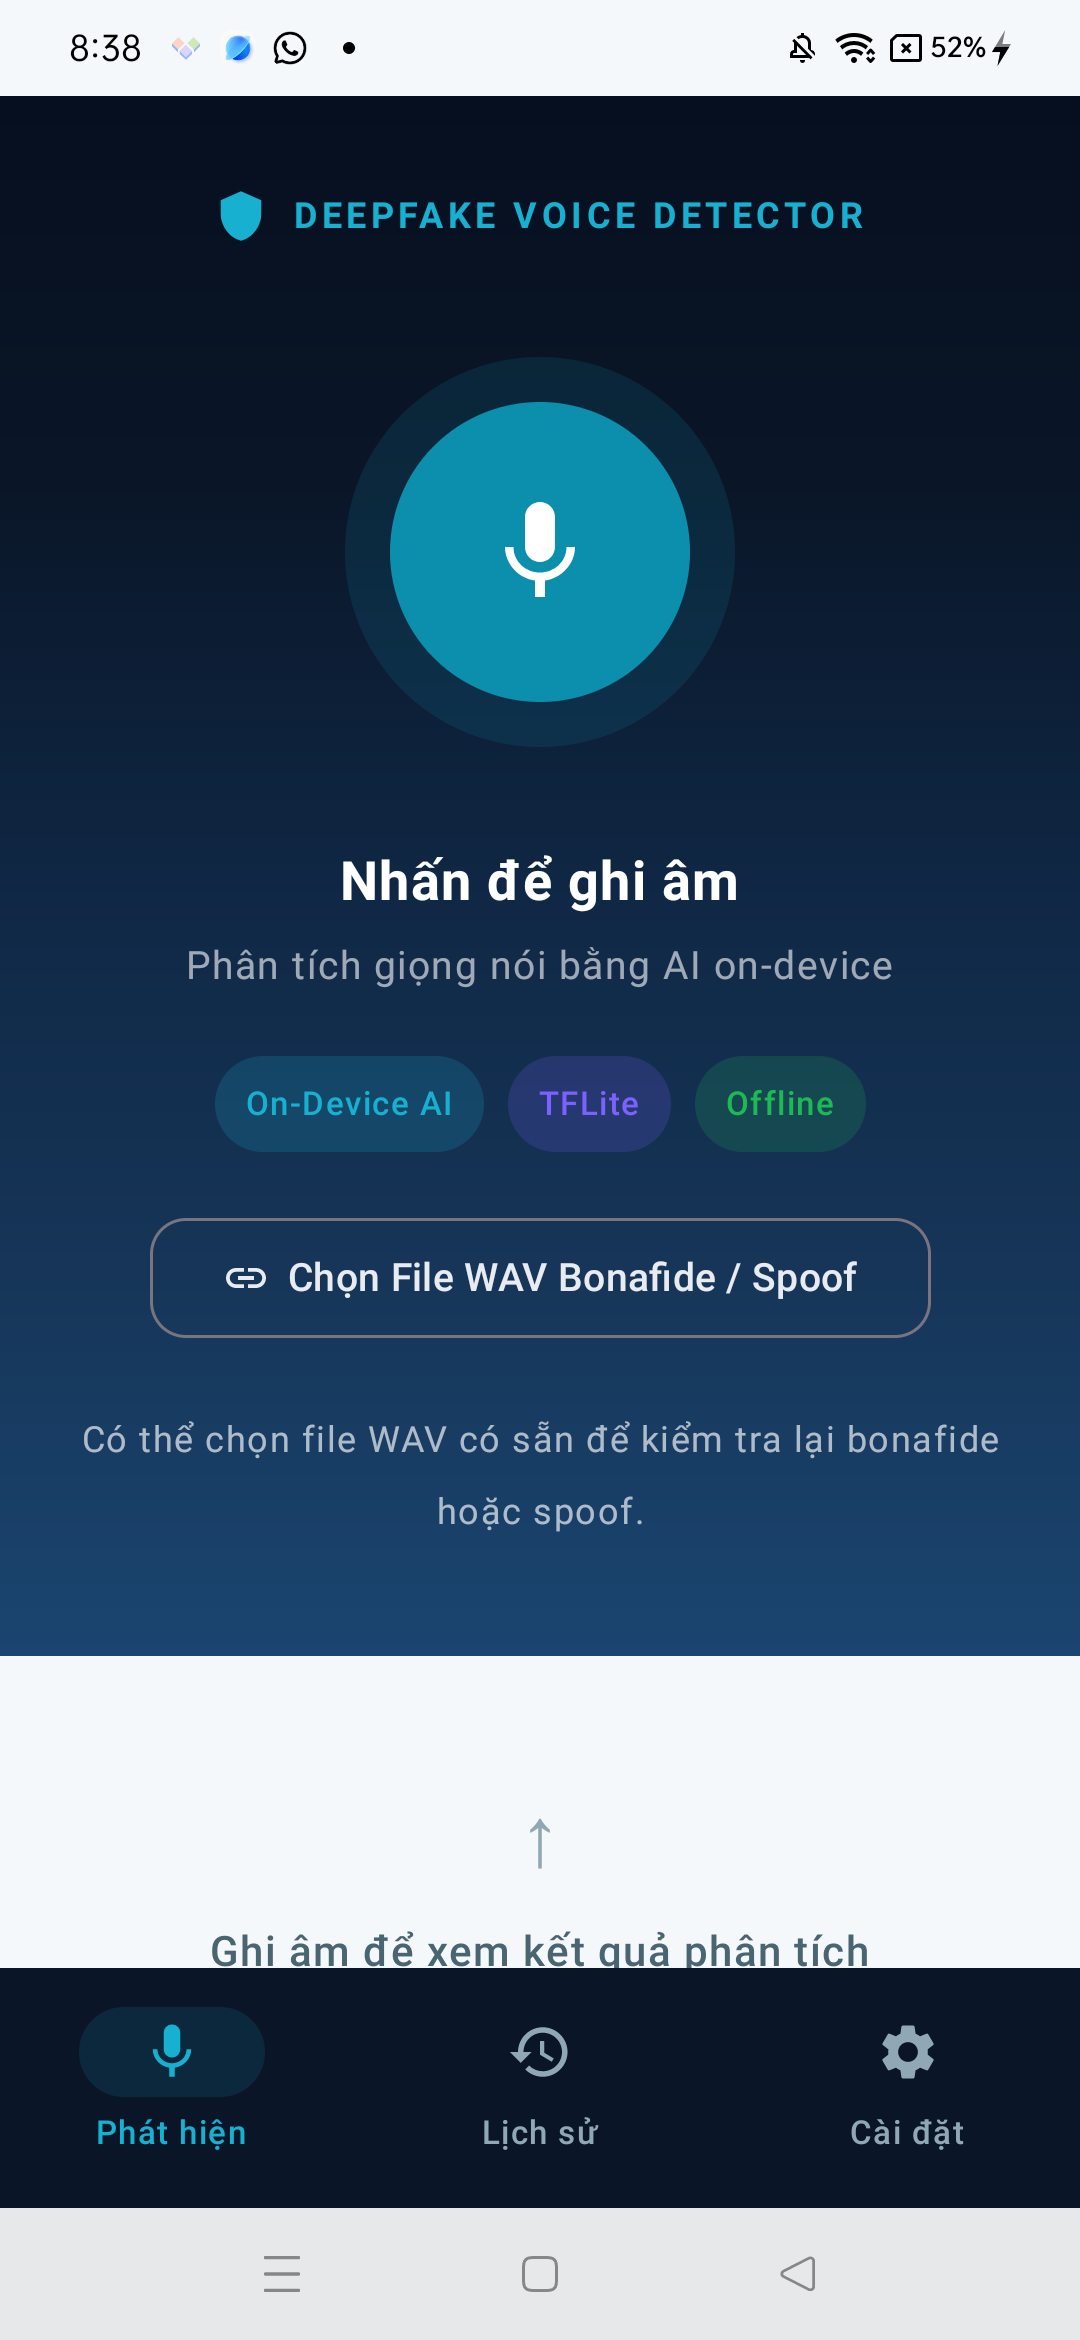
\includegraphics[width=\linewidth]{01_detect_current.png}
\end{minipage}
\hfill
\begin{minipage}{0.48\columnwidth}
    \centering
    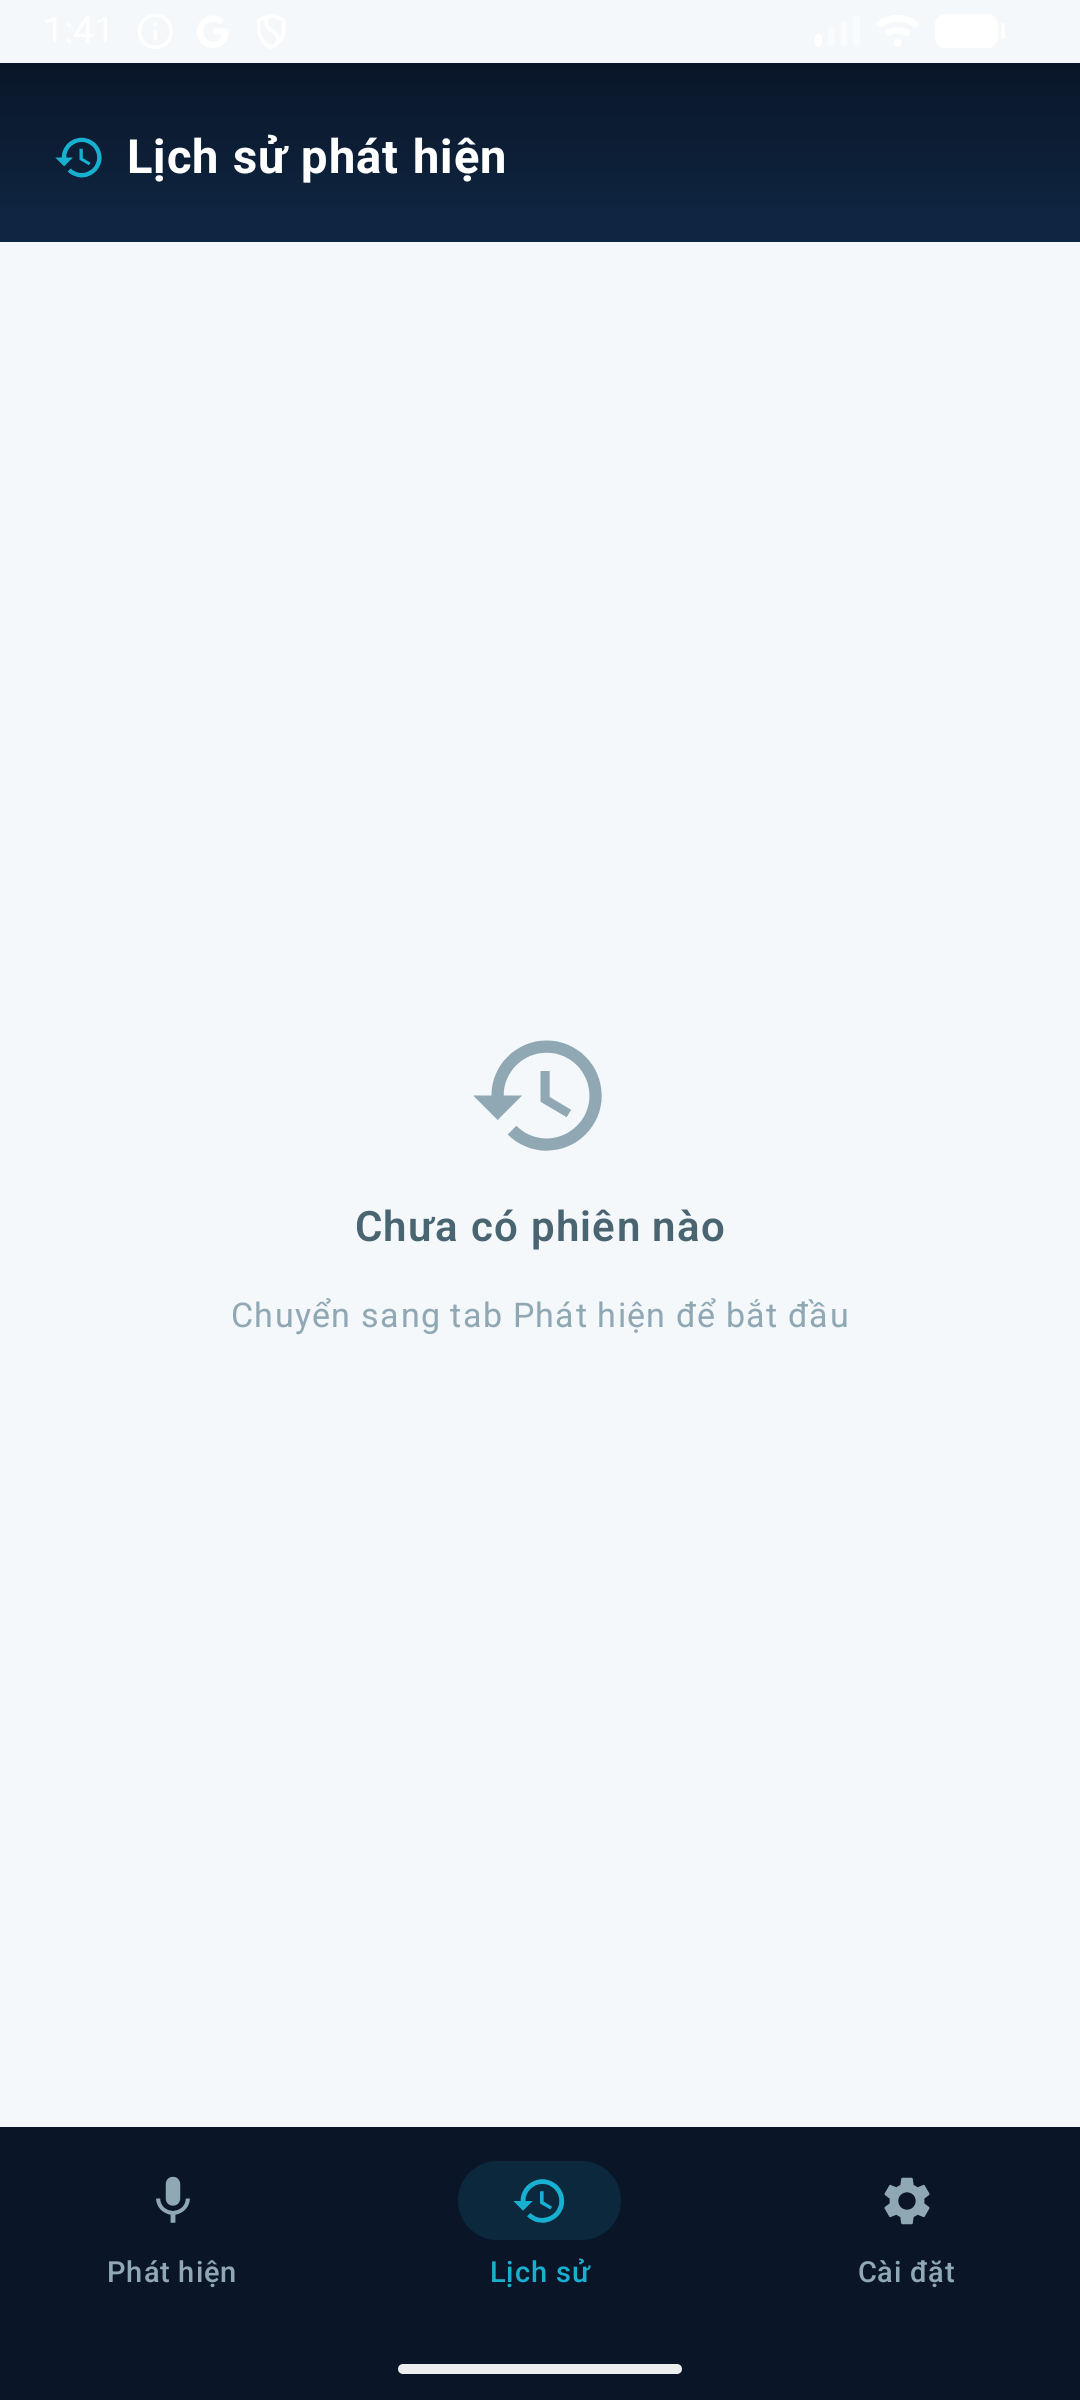
\includegraphics[width=\linewidth]{02_history_empty_current.png}
\end{minipage}
\\[4pt]
\includegraphics[width=0.78\columnwidth]{fig_confusion_matrix.png}
\caption{Current Android UI states and the confusion matrix of Cross-Scale Attention Lite on the 1{,}700-sample external holdout.}
\label{fig:runtime-figs}
\end{figure}

The current study also has clear limitations. First, the external holdout is still relatively small at 1{,}700 samples, so broader microphone, environment, and synthesis diversity would strengthen the claims. Second, the threshold is fixed globally; an adaptive threshold or risk-aware decision policy could reduce FAR without collapsing recall. Third, DynamicRange appears weak on the internal ablation, so future work should re-evaluate whether it truly helps out-of-domain robustness or can be replaced with a more stable mobile feature.

\section{Conclusion}

This paper presented a lightweight Vietnamese speech anti-spoofing pipeline designed specifically for Android deployment. By combining eight handcrafted acoustic features, a compact Cross-Scale Attention Lite classifier, and selective mixing of only 150 external samples per class, the system generalizes well enough to reach 85.29\% external accuracy and 97.65\% spoof recall while remaining small enough for direct mobile integration.

Beyond model accuracy, the project demonstrates an end-to-end deployment story: the detector is exported to TensorFlow Lite, integrated into an Android application, exposed through practical user flows, and measured directly in terms of runtime latency and RAM usage. These results show that Vietnamese anti-spoofing does not necessarily require large server-side models to be useful in practice.

Future work should expand the external dataset, validate on a wider range of real devices and microphones, and explore threshold adaptation or additional low-cost features to reduce false acceptance while preserving high spoof recall. Even in its current form, the proposed system provides a credible baseline for privacy-preserving, on-device anti-spoofing in Vietnamese mobile applications.

\begin{thebibliography}{00}

\bibitem{b1} X. Wang, J. Yamagishi, M. Todisco, H. Delgado, N. Evans, T. Kinnunen, K.-A. Lee, V. Vestman, A. Nautsch, H. Sahidullah, M. Diez, F. Alegre, and M. A. Patel, ``ASVspoof 2019: A large-scale public database of synthesized, converted and replayed speech,'' \emph{Computer Speech \& Language}, vol. 64, 2020.

\bibitem{b2} J.-W. Jung, H.-S. Heo, H.-J. Shim, H.-J. Yu, and H.-M. Yu, ``AASIST: Audio anti-spoofing using integrated spectro-temporal graph attention networks,'' in \emph{Proc. IEEE ICASSP}, 2022, pp. 6367--6371.

\bibitem{b3} H. Tak, J. Patino, M. Todisco, A. Nautsch, N. W. D. Evans, and A. Larcher, ``End-to-end anti-spoofing with RawNet2,'' in \emph{Proc. IEEE ICASSP}, 2021, pp. 6369--6373.

\bibitem{b4} H. Tak, J. Patino, M. Todisco, A. Nautsch, N. W. D. Evans, and A. Larcher, ``RawBoost: A raw data boosting and augmentation method applied to automatic speaker verification anti-spoofing,'' in \emph{Proc. IEEE ICASSP}, 2022, pp. 6382--6386.

\bibitem{b5} Google, ``TensorFlow Lite for mobile and edge devices,'' accessed Jul. 3, 2026. [Online]. Available: \url{https://www.tensorflow.org/lite}

\end{thebibliography}

\end{document}
